\section{Sampling the auxiliary polynomial}\label{sec:sampling}

We now prove Proposition~\ref{prop:almost-signs}.  The auxiliary polynomial
from Proposition~\ref{prop:auxiliary} has nearly full mean-square mass, and
each Fourier coefficient has a prescribed admissible width.  We pack those
widths, then sample the polynomial along quadratic paths on consecutive
blocks.  The packing allows only one stationary contribution at any angle;
the distinct packed centers also preserve the mean-square mass when some
curvatures coincide.

\subsection{A uniform estimate for quadratic sums}

Bombieri and Bourgain \cite[Section~7]{BombieriBourgain2009} use Poisson
summation to evaluate smoothed quadratic phases in their unimodular
construction.  The next lemma isolates the uniformity needed here for
the maximum over the whole circle.  Its data are fixed while the integer
$N$ tends to infinity.

\begin{lemma}\label{lem:sampling-poisson}
Let $\chi\in C_c^\infty(\R)$, let $x_*\in\R$ and
$\lambda\in\R\setminus\{0\}$, and let $J\subset\R$ be compact.
For $b\in J$ and $\ell\in\Z$, put
\[
 x_{b,\ell}=x_*+\frac{\ell-b}{\lambda},
 \qquad
 \omega_{b,\ell}=(b-\ell)x_*
                  -\frac{(b-\ell)^2}{2\lambda}.
\]
As $N$ tends to infinity through positive integers, uniformly for $b\in J$,
\begin{align}
 &\frac1{\sqrt N}\sum_{k\in\Z}\chi(k/N)
   \e\!\left(bk+\frac{N\lambda}{2}(k/N-x_*)^2\right)
 \notag\\
 &\qquad=
 \frac1{\sqrt{|\lambda|}}
 \sum_{\ell\in\Z}\chi(x_{b,\ell})
 \e\!\left(\frac{\operatorname{sgn}\lambda}{8}
                      +N\omega_{b,\ell}\right)
 +O(N^{-1}).\label{eq:sampling-poisson}
\end{align}
The sum on the right has only finitely many nonzero terms, lying in one
fixed finite set of indices for all $b\in J$.  The error constant depends
only on the fixed data $\chi,x_*,\lambda,J$.
\end{lemma}

\begin{proof}
For $b\in J$ and $\ell\in\Z$, define
\[
 \phi_{b,\ell}(x)
   =\frac{\lambda}{2}(x-x_*)^2+(b-\ell)x.
\]
Poisson summation, with the change of variable $k/N$, gives
\begin{align}
 &\frac1{\sqrt N}\sum_{k\in\Z}\chi(k/N)
   \e\!\left(bk+\frac{N\lambda}{2}(k/N-x_*)^2\right)
 \notag\\
 &\hspace{35mm}=
 \sqrt N\sum_{\ell\in\Z}
       \int_{\R}\chi(x)\e\!\left(N\phi_{b,\ell}(x)\right)\,dx.
 \label{eq:sampling-poisson-identity}
\end{align}
Here the factor $N$ from Poisson summation combines with the original
factor $N^{-1/2}$ to give $\sqrt N$.

Choose a fixed integer $L$ so large that, for $|\ell|>L$,
\[
 |\phi'_{b,\ell}(x)|
   =|\lambda(x-x_*)+b-\ell|\ge |\ell|/2
\]
on $\operatorname{supp}\chi$, uniformly in $b\in J$.  Since the amplitude
is compactly supported, two integrations by parts have no boundary terms
and yield
\begin{align*}
 \int\chi\,\e(N\phi_{b,\ell})
  =\frac1{(2\pi iN)^2}\int
  \left\{
   \frac{\chi''}{(\phi'_{b,\ell})^2}
   -\frac{3\lambda\chi'}{(\phi'_{b,\ell})^3}
   +\frac{3\lambda^2\chi}{(\phi'_{b,\ell})^4}
  \right\}\e(N\phi_{b,\ell}).
\end{align*}
These integrals are $O(N^{-2}|\ell|^{-2})$.  Their total contribution to
\eqref{eq:sampling-poisson-identity} is therefore $O(N^{-3/2})$, uniformly
in $b$.  This summable estimate handles the infinite tail before any
stationary-phase errors are added.

For the finitely many indices $|\ell|\le L$, expand the phase as
\[
 N\phi_{b,\ell}(x)
 =\frac{N\lambda x^2}{2}
   -N(\ell-b+\lambda x_*)x+\frac{N\lambda x_*^2}{2}.
\]
Apply Lemma~\ref{lem:quadratic} with $T=N$, curvature $\lambda$, and
$u=N(\ell-b+\lambda x_*)$.  Its stationary point is $x_{b,\ell}$, and
$\phi_{b,\ell}(x_{b,\ell})=\omega_{b,\ell}$.  After multiplication by
$\sqrt N$, it gives the corresponding term in
\eqref{eq:sampling-poisson} with error $O(N^{-1})$, uniformly in $b$.
Increasing $L$ if necessary ensures
$\chi(x_{b,\ell})=0$ whenever $|\ell|>L$ and $b\in J$.
Summing the finitely many remaining errors proves the lemma.
\end{proof}

\subsection{Fixed blocks and separated stationary contributions}

\begin{proof}[Proof of Proposition~\ref{prop:almost-signs}]
Fix $0<\delta<1/20$.  Proposition~\ref{prop:auxiliary} supplies a real
trigonometric polynomial on $\T^m$,
\[
 F(y)=\sum_{a\in\mathcal A}c_a\e(a\cdot y),
 \qquad c_a=\widehat F(a),
 \qquad \mathcal A=\{\pm a_i:1\le i\le r\},
\]
and a vector $v\in\R^m$.  The representatives $a_i$ are nonzero and
pairwise nonparallel.  Write $\lambda_a=a\cdot v$.  The properties needed
here are
\begin{gather}
 \norm{F}_\infty\le1,\qquad
 \norm{F}_2\ge1-3\delta,\qquad
 \lambda_a\ne0,\qquad
 \sum_{a\in\mathcal A}|\lambda_a|<1,
 \label{eq:sampling-auxiliary-budgets}\\
 \frac{|c_a|}{\sqrt{|\lambda_a|}}\le K_\delta
 \quad(a\in\mathcal A).
 \label{eq:sampling-coefficient-budget}
\end{gather}
The set $\mathcal A$ is a containing Fourier support; coefficients equal
to zero are allowed.

Apply Lemma~\ref{lem:signed-packing} with $w_i=|\lambda_{a_i}|$.
Its strict width hypothesis holds because
$2\sum_i w_i=\sum_{a\in\mathcal A}|\lambda_a|<1$.
We obtain an integer $H\ge1$ and points $\theta_h\in\T^m$ such that all
the closed intervals
\begin{equation}\label{eq:sampling-packed-intervals}
 I_{a,h}=a\cdot\theta_h+
 \left[-\frac{|\lambda_a|}{2H},
             \frac{|\lambda_a|}{2H}\right]\pmod1,
 \qquad a\in\mathcal A,\quad 1\le h\le H,
\end{equation}
are pairwise disjoint.  Each has length less than one.

Put $x_h^*=(h-1/2)/H$.  Choose smooth cutoffs
\[
 \chi_h\in C_c^\infty\!\left((h-1)/H,h/H\right),\qquad
 0\le\chi_h\le1,\qquad
 \sum_{h=1}^H\int_{\R}\chi_h(x)^2\,dx\ge1-\delta.
\]
Such cutoffs can be chosen to equal one except in sufficiently small
neighborhoods of the block endpoints.  All data chosen so far, including
the cutoffs, are now fixed independently of $N$.

For every integer $N\ge1$ and $0\le k<N$, define
\begin{equation}\label{eq:sampling-coefficients}
 X_{N,k}=
 \sum_{h=1}^H\chi_h(k/N)
 F\!\left(k\theta_h+\frac N2v(k/N-x_h^*)^2\right).
\end{equation}
The expression does not depend on the choice of real lifts of
$\theta_h$.  It is real, and at most one summand is nonzero, so
$|X_{N,k}|\le1$.  As every cutoff is supported strictly inside $(0,1)$,
extending the sum over $k$ to all integers introduces no additional
nonzero terms.

\paragraph{The maximum on the whole circle.}
Expand $F$ in \eqref{eq:sampling-coefficients} and apply
Lemma~\ref{lem:sampling-poisson} with
\[
 b=t+a\cdot\theta_h,\qquad
 \lambda=\lambda_a,\qquad x_*=x_h^*,\qquad \chi=\chi_h.
\]
For fixed real lifts of the finitely many $\theta_h$, all such $b$ lie in
one compact interval as $t$ ranges over $[0,1]$.  Thus every error is
uniform in $t$.  The leading term indexed by $(a,h,\ell)$ contains
\begin{equation}\label{eq:sampling-stationary-point}
 \chi_h\!\left(x_h^*+\frac{\ell-t-a\cdot\theta_h}{\lambda_a}\right).
\end{equation}
\begin{samepage}
For this factor to be nonzero, its argument must lie in the interior of
the $h$th block.  Hence
\[
 |\ell-t-a\cdot\theta_h|<\frac{|\lambda_a|}{2H},
\]
which says that $-t\pmod1$ lies in $I_{a,h}$, as illustrated in
Figure~\ref{fig:sampling-intervals}.
\end{samepage}

Disjointness of all intervals in \eqref{eq:sampling-packed-intervals}
allows at most one pair $(a,h)$.  For that pair, their length being less
than one allows at most one integer $\ell$.  The cutoffs vanish near block
endpoints, so this argument also covers angles at the ends of the packed
intervals.

\begin{figure}[H]
\centering
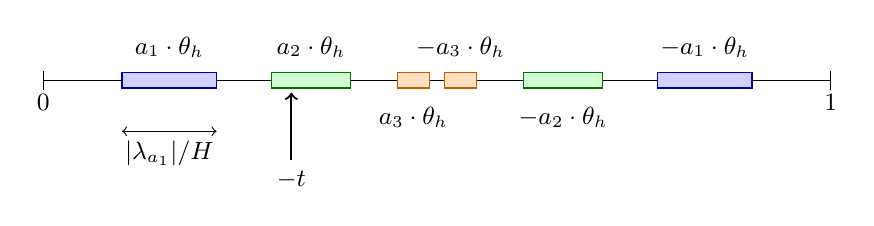
\begin{tikzpicture}[x=1cm,y=1cm,font=\small]
 \draw (0,0)--(10,0);
 \draw (0,-.12)--(0,.12) node[below=5pt] {$0$};
 \draw (10,-.12)--(10,.12) node[below=5pt] {$1$};
 \filldraw[fill=blue!18,draw=blue!65!black] (1,-.10) rectangle (2.2,.10);
 \filldraw[fill=blue!18,draw=blue!65!black] (7.8,-.10) rectangle (9,.10);
 \filldraw[fill=green!18,draw=green!45!black] (2.9,-.10) rectangle (3.9,.10);
 \filldraw[fill=green!18,draw=green!45!black] (6.1,-.10) rectangle (7.1,.10);
 \filldraw[fill=orange!25,draw=orange!75!black] (4.5,-.10) rectangle (4.9,.10);
 \filldraw[fill=orange!25,draw=orange!75!black] (5.1,-.10) rectangle (5.5,.10);
 \node at (1.6,.42) {$a_1\cdot\theta_h$};
 \node at (3.4,.42) {$a_2\cdot\theta_h$};
 \node at (4.7,-.47) {$a_3\cdot\theta_h$};
 \node at (5.3,.42) {$-a_3\cdot\theta_h$};
 \node at (6.6,-.47) {$-a_2\cdot\theta_h$};
 \node at (8.4,.42) {$-a_1\cdot\theta_h$};
 \draw[->,thick] (3.15,-1.02) node[below] {$-t$} -- (3.15,-.16);
 \draw[<->] (1,-.65)--(2.2,-.65)
    node[midway,below] {$|\lambda_{a_1}|/H$};
\end{tikzpicture}
\caption{Schematic signed intervals for one block, drawn in a representative
of $\T$.  Paired intervals have the same width and opposite centers.  The
construction packs the intervals for every block together.  Only an interval
containing $-t$ can give a nonzero stationary contribution at angle $t$;
the diagram illustrates this condition, not a particular packing produced
by the lemma.}
\label{fig:sampling-intervals}
\end{figure}

By \eqref{eq:sampling-coefficient-budget}, the modulus of the sole
possible leading contribution, including its Fourier coefficient, is at
most $K_\delta$.  Summing the errors over the fixed finite set of pairs
$(a,h)$ therefore gives
\begin{equation}\label{eq:sampling-uniform-maximum}
 \frac1{\sqrt N}\max_{t\in\T}
 \left|\sum_{k=0}^{N-1}X_{N,k}\e(kt)\right|
 \le K_\delta+o(1).
\end{equation}
The error tends to zero uniformly in $t$, with all construction data held
fixed.  We have obtained the desired maximum bound; it remains to show
that sampling retains the mean-square mass of $F$.

\paragraph{The mean-square mass.}
The block supports are disjoint, so products from different blocks vanish.
Within block $h$, a pair $a,a'\in\mathcal A$ contributes the coefficient
$c_a\overline{c_{a'}}$ times
\begin{equation}\label{eq:sampling-energy-term}
 \frac1N\sum_{k\in\Z}\chi_h(k/N)^2
 \e\!\left(k\beta+\frac{N\kappa}{2}(k/N-x_h^*)^2\right),
 \quad
 \beta=(a-a')\cdot\theta_h,\quad
 \kappa=\lambda_a-\lambda_{a'}.
\end{equation}
If $a=a'$, this is a Riemann sum with limit $\int\chi_h^2$.
If $\kappa\ne0$, Lemma~\ref{lem:sampling-poisson}, now with amplitude
$\chi_h^2$, shows that the sum with normalization $N^{-1/2}$ is bounded.
The additional factor $N^{-1/2}$ in \eqref{eq:sampling-energy-term}
therefore makes this contribution tend to zero.

The remaining case is $a\ne a'$ and $\kappa=0$.  It cannot be omitted:
the coefficient-spreading construction deliberately produces repeated
curvatures.  The centers of $I_{a,h}$ and $I_{a',h}$ are distinct modulo
one, so $\beta\notin\Z$.  Geometric summation gives
\[
 \left|\sum_{k=u}^{w}\e(k\beta)\right|
 \le\frac2{|1-\e(\beta)|}\qquad(u,w\in\Z,\ u\le w).
\]
Writing $\psi=\chi_h^2$, summation by parts consequently bounds
$\sum_k\psi(k/N)\e(k\beta)$ by a fixed constant times
$\norm{\psi}_\infty+\int|\psi'|$.  Indeed the discrete variation is at
most $\int|\psi'|$.  Division by $N$ again makes
\eqref{eq:sampling-energy-term} tend to zero.

\begin{samepage}
There are only finitely many pairs, so we may sum these limits.  Parseval
on the auxiliary torus gives
\begin{align}
 \lim_{N\to\infty}\frac1N\sum_{k=0}^{N-1}X_{N,k}^2
 &=\left(\sum_{h=1}^H\int\chi_h^2\right)
            \sum_{a\in\mathcal A}|c_a|^2
 \notag\\
 &=\left(\sum_{h=1}^H\int\chi_h^2\right)\norm{F}_2^2
 \notag\\
 &\ge(1-\delta)(1-3\delta)^2
   =1-7\delta+15\delta^2-9\delta^3
   \ge1-7\delta.\label{eq:sampling-energy-limit}
\end{align}
\end{samepage}
Together with \eqref{eq:sampling-uniform-maximum}, this proves
Proposition~\ref{prop:almost-signs}.
Every integer $N$ was allowed throughout.  In particular, neither the
packing prime nor the number of blocks imposes a divisibility condition
on $N$.
\end{proof}
